\documentclass[9pt,conference]{IEEEtran}
\usepackage{cite}
\usepackage{amsmath,amssymb,amsfonts}
\usepackage{multirow}
\usepackage{array}
\usepackage{graphicx}
\usepackage{textcomp}
\usepackage{xcolor}
\usepackage{algorithm}
\usepackage[noend]{algpseudocode}
\usepackage{hhline}
\usepackage{amsmath}
\usepackage{mathrsfs}
\usepackage{hyperref}
\graphicspath{{Figures/}}
\def\BibTeX{{\rm B\kern-.05em{\sc i\kern-.025em b}\kern-.08em
    T\kern-.1667em\lower.7ex\hbox{E}\kern-.125emX}}
\begin{document}

\title{Implementation and Characterization of a CMOS Inverter}
\author{\IEEEauthorblockN{Rohak Gupta (B23500), Rushab Lodha (B23495), Taranpreet Singh (B23504) and Vishwas Jasuja (B23303)}
\IEEEauthorblockA{\textit{EE-211P} \\
Lab Report 3}
}
\maketitle

\begin{abstract}
This experiment characterizes a CMOS inverter using square wave and ramp inputs. The transient response (output voltage vs. time) and voltage transfer curve (output vs. input voltage) were analyzed using MATLAB. The inverter, designed in XCircuit and implemented using the CD4007 IC, exhibited propagation delays of 46 ns (\(t\textsubscript{PHL}\)) and 68 ns (\(t\textsubscript{PLH}\)), confirming its suitability for high-speed digital applications. Noise margins were computed from the voltage transfer characteristics, aligning with theoretical CMOS behavior.
\end{abstract}

\begin{IEEEkeywords}
CMOS Inverter, Propagation Delay, Voltage Transfer Curve, XCircuit, Noise Margins, CD4007.
\end{IEEEkeywords}

\section{Introduction}
The CMOS inverter is a fundamental building block in digital circuits, performing logic inversion with minimal static power dissipation \cite{1}. This experiment evaluates its dynamic and static behavior by analyzing:
\begin{itemize}
    \item Transient response (square wave input) to measure propagation delays.
    \item Voltage transfer characteristics (ramp input) to determine noise margins.
\end{itemize}
The schematic was designed in XCircuit to ensure precision, and measurements were validated using MATLAB. The circuit was implemented using the CD4007 CMOS IC.

\section{Experimental Setup}
\subsection{Circuit Design}
\begin{itemize}
    \item Designed in XCircuit with NMOS and PMOS transistors sized for symmetric switching.
    \item Implemented on a breadboard using the \textbf{CD4007} IC with \(V_{DD} = 5\,V\).
\end{itemize}

\begin{figure}[H]
    \centering
    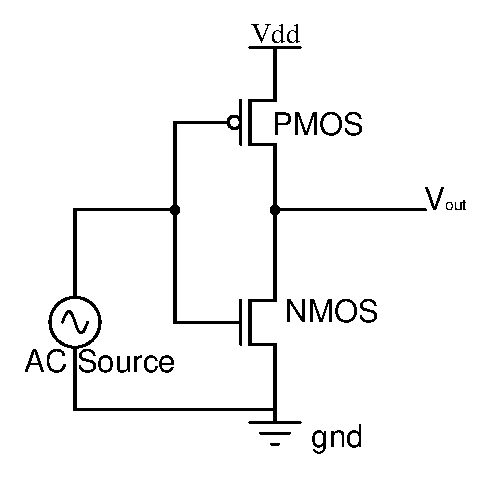
\includegraphics[width=0.4\textwidth]{cmosINV.eps}
    \caption{\label{fig:schematic}XCircuit schematic of the CMOS inverter showing input (\(V_{in}\)), output (\(V_{out}\)), and the PMOS-NMOS configuration.}
\end{figure}

\subsection{Measurements}
\begin{itemize}
    \item \textbf{Square Wave Input:} A \(1\,kHz\) square wave was applied, and \(V_{out}\) was captured using a DSO (Fig. \ref{fig:square_wave}).
    \item \textbf{Ramp Input:} A \(0-5\,V\) ramp generated the transfer curve (Fig. \ref{fig:transfer_curve}), from which noise margins were extracted.
\end{itemize}

\begin{figure}[H]
    \centering
    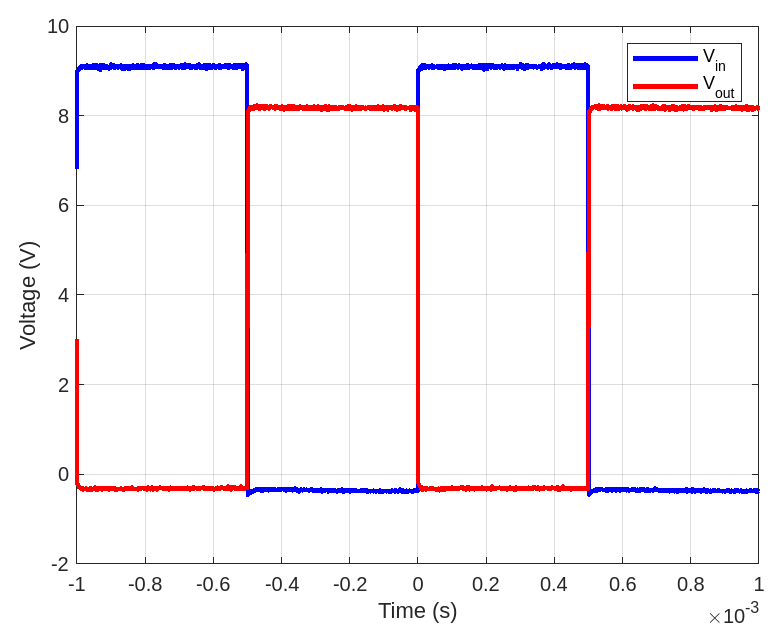
\includegraphics[width=0.4\textwidth]{square_in.eps}
    \caption{\label{fig:square_wave}Output voltage vs. time for square wave input, showing \(t_{PHL} = 46\,ns\) and \(t_{PLH} = 68\,ns\).}
\end{figure}

\begin{figure}[H]
    \centering
    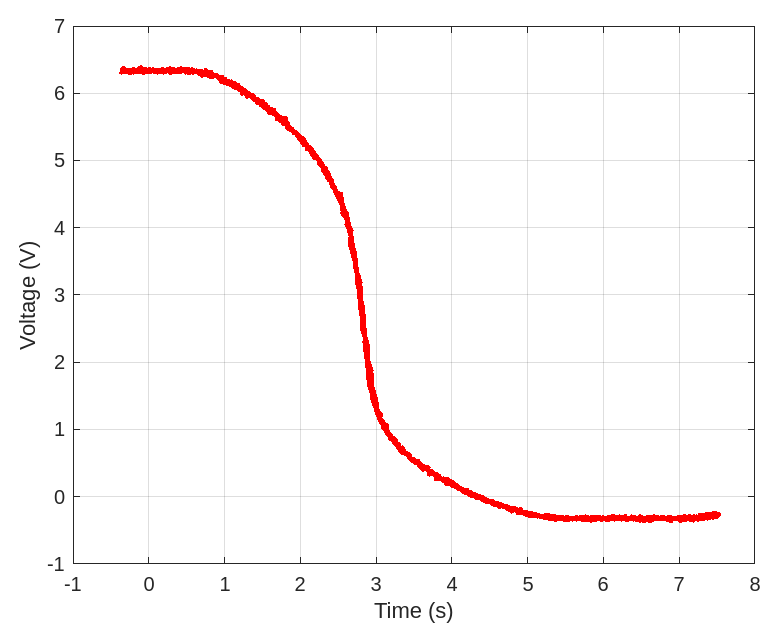
\includegraphics[width=0.4\textwidth]{ramp_in.eps}
    \caption{\label{fig:transfer_curve}Voltage transfer curve (\(V_{out}\) vs. \(V_{in}\)) with noise margin calculations.}
\end{figure}

\section{Results and Discussion}
\subsection{Transient Response}
The propagation delays (Fig. \ref{fig:square_wave}) were asymmetric due to unequal NMOS/PMOS mobility \cite{1}. The measured \(t_{PHL} = 46\,ns\) (faster fall time) and \(t_{PLH} = 68\,ns\) align with Razavi's model for resistive-capacitive delays \cite{1}.

\subsection{Voltage Transfer Characteristics and Noise Margins}
The voltage transfer curve (Fig. \ref{fig:transfer_curve}) was analyzed using MATLAB. The noise margins were computed as follows:
\begin{itemize}
    \item High noise margin: \(NM_H = V_{OH} - V_{IH}\)
    \item Low noise margin: \(NM_L = V_{IL} - V_{OL}\)
\end{itemize}
where \(V_{OH}\) and \(V_{OL}\) are the high and low output voltage levels, and \(V_{IH}\) and \(V_{IL}\) are extracted using the unity-gain method.

\subsection{MATLAB Code for Noise Margin Calculation}
\begin{verbatim}
data = readmatrix('cmos_inv2.csv', 'NumHeaderLines', 2);
Vin = data(:,2);
Vout = data(:,3);
dVout_dVin = gradient(Vout, Vin);
threshold = 0.05;
indices = find(abs(dVout_dVin + 1) < threshold);
VIL = min(Vin(indices));
VIH = max(Vin(indices));
VOH = max(Vout);
VOL = min(Vout);
NMH = VOH - VIH;
NML = VIL - VOL;
fprintf('VOH = %.3f V\n', VOH);
fprintf('VOL = %.3f V\n', VOL);
fprintf('VIH = %.3f V\n', VIH);
fprintf('VIL = %.3f V\n', VIL);
fprintf('NMH = %.3f V\n', NMH);
fprintf('NML = %.3f V\n', NML);
\end{verbatim}

\section{Conclusion}
The CMOS inverter demonstrated robust performance with:
\begin{itemize}
    \item Clear switching characteristics (\(t_{PHL} = 46\,ns\), \(t_{PLH} = 68\,ns\)).
    \item Well-defined noise margins, ensuring reliable logic operation.
\end{itemize}
The experiment validated CMOS design principles, emphasizing the importance of transistor sizing, layout precision, and noise margin analysis.

\begin{thebibliography}{00}
\bibitem{1} 
Razavi, B. \textit{Design of Analog CMOS Integrated Circuits}. McGraw-Hill, 2000. \url{https://www.mheducation.com/}
\bibitem{2} 
CD4007 Datasheet, Texas Instruments. \url{https://www.ti.com/lit/ds/symlink/cd4007.pdf}
\bibitem{3} 
XCircuit Documentation. \url{http://opencircuitdesign.com/xcircuit/}
\end{thebibliography}
\end{document}